\begin{center}
	\begin{tabular}{M{9.25cm}M{8.75cm}}
		\textbf{TRƯỜNG THCS-THPT NGUYỄN KHUYẾN}& \textbf{ÔN TẬP KTTX LẦN 2 - HỌC KÌ II}\\
		\textbf{MÃ ĐỀ: 001}& \textbf{Bài thi môn: VẬT LÝ 10}\\
		\textit{(Đề thi có 04 trang)}& \textit{Thời gian làm bài: 45 phút, không kể phát đề}
		
		\noindent\rule{4cm}{0.8pt} \\
	\end{tabular}
\end{center}
\begin{center}
	\textit{Lấy gia tốc rơi tự do $g=\SI{10}{\meter/\second^2}$; khối lượng riêng của nước $\rho=\SI{1000}{\kilogram/\meter^3}$; $\SI{1}{HP}=\SI{746}{\watt}$.}
\end{center}
\setcounter{section}{0}
\section{Câu trắc nghiệm nhiều phương án lựa chọn}
\textit{Thí sinh trả lời từ câu 1 đến câu 12. Mỗi câu hỏi thí sinh chọn một phương án}
\setcounter{ex}{0}
\Opensolutionfile{ans}[ans/D10-KTTX2-HK2-TN]
% ===================================================================
\begin{ex}
	Công suất được xác định bằng
	\choice
	{\True công thực hiện trong một đơn vị thời gian}
	{công thực hiện trong đơn vị dài}
	{tích của công và thời gian thực hiện công}
	{tổng độ lớn công phát động}
	\loigiai{}
\end{ex}
% ===================================================================
\begin{ex}
	Trong ô tô, xe máy, \dots có bộ phận hộp số (sử dụng các bánh xe truyền động có bán kính to nhỏ khác nhau) nhằm mục đích
	\choice
	{thay đổi công suất của xe}
	{\True thay đổi lực phát động của xe}
	{thay đổi công của xe}
	{duy trì vận tốc không đổi của xe}
	\loigiai{}
\end{ex}
% ===================================================================
\begin{ex}
	Một quả bóng được ném tung lên cao từ mặt đất, sau đó rơi trở lại đất. Công của trọng lực trong suốt quá trình này bằng
	\choice
	{$mgh$}
	{\True $0$}
	{$2mgh$}
	{không xác định được}
	\loigiai{}
\end{ex}
% ===================================================================
\begin{ex}
	Một ô tô đang chạy trên đường với tốc độ \SI{72}{\kilo\meter/\hour}. Công suất của động cơ là \SI{60}{\kilo\watt}. Lực phát động của động cơ là
	\choice
	{\SI{2500}{\newton}}
	{\True \SI{3000}{\newton}}
	{\SI{2800}{\newton}}
	{\SI{1550}{\newton}}
	\loigiai{}
\end{ex}
% ===================================================================
\begin{ex}
Một vật có khối lượng $m=\SI{100}{\gram}$ trượt xuống mặt phẳng nghiêng dài \SI{3}{\meter} và nghiêng \SI{30}{\degree} so với phương ngang. Công của trọng lực tác dụng lên vật là
	\choice
	{\True \SI{1.5}{\joule}}
	{\SI{-1.5}{\joule}}
	{\SI{3}{\joule}}
	{\SI{-3}{\joule}}
	\loigiai{}
\end{ex}
% ===================================================================
\begin{ex}
	Một máy bơm nước mỗi giây có thể bơm \SI{15}{\liter} nước lên bể nước ở độ cao \SI{10}{\meter}. Nếu coi tổn hao là không đáng kể. Công suất của máy bơm là
	\choice
	{\SI{150}{\watt}}
	{\SI{3000}{\watt}}
	{\True \SI{1500}{\watt}}
	{\SI{2000}{\watt}}
	\loigiai{}
\end{ex}
% ===================================================================
\begin{ex}
	Một lực kéo \SI{2500}{\newton} theo phương ngang tác dụng lên một chiếc xe khối lượng \SI{500}{\kilogram} đang đứng yên trên mặt đường nằm ngang. Biết tổng lực cản tác dụng lên xe có độ lớn \SI{1000}{\newton}. Công của lực kéo tác dụng lên xe khi xe chuyển động được \SI{2}{\second} là 
	\choice
	{\SI{6}{\kilo\joule}}
	{\SI{9}{\kilo\joule}}
	{\True \SI{15}{\kilo\joule}}
	{\SI{21}{\kilo\joule}}
	\loigiai{}
\end{ex}
% ===================================================================
\begin{ex}
	Một dây cáp sử dụng động cơ điện tạo ra một lực không đổi \SI{50}{\newton} tác dụng lên vật và kéo vật đi một đoạn đường \SI{30}{\meter} trong thời gian \SI{1}{\minute}. Công suất của động cơ là
	\choice
	{\SI{50}{\watt}}
	{\True \SI{25}{\watt}}
	{\SI{100}{\watt}}
	{\SI{75}{\watt}}
	\loigiai{}
\end{ex}
% ===================================================================
\begin{ex}
	Một động cơ điện được thiết kế để kéo thùng than nặng \SI{400}{\kilogram} từ dưới mỏ có độ sâu \SI{200}{\meter} lên mặt đất trong thời gian \SI{2}{\minute}. Hiệu suất của động cơ là \SI{80}{\percent}. Công suất toàn phần của động cơ là
	\choice
	{\True \SI{8.3}{\kilo\watt}}
	{\SI{6.6}{\kilo\watt}}
	{\SI{83}{\kilo\watt}}
	{\SI{66}{\kilo\watt}}
	\loigiai{}
\end{ex}
% ===================================================================
\begin{ex}
	Một động cơ có công suất tiêu thụ bằng $\SI{5}{\kilo\watt}$ kéo một vật có trọng lượng $\SI{12}{\kilo\newton}$ lên cao $\SI{30}{\meter}$ theo phương thẳng đứng trong thời gian $\SI{90}{\second}$ với vận tốc không đổi. Hiệu suất của động cơ bằng
	\choice
	{$\SI{100}{\percent}$}
	{\True $\SI{80}{\percent}$}
	{$\SI{60}{\percent}$}
	{$\SI{40}{\percent}$}
	\loigiai{Công cần thiết để kéo vật nặng lên cao $\SI{30}{\meter}$:
		$$A_i=Ph=\SI{360}{\kilo\joule}$$
		Công suất có ích để kéo vật:
		$$\calP_i=\dfrac{A_i}{t}=\SI{40}{\kilo\watt}$$
		Hiệu suất động cơ:
		$$H=\dfrac{\calP_i}{\calP_{tp}}\cdot\SI{100}{\percent}=\SI{80}{\percent}.$$}
\end{ex}
% ===================================================================
\begin{ex}
	Một người nhấc một vật có khối lượng \SI{5}{\kilogram} lên độ cao \SI{1.2}{\meter} rồi mang đi ngang một đoạn \SI{50}{\meter}. Công tổng cộng mà người này đã thực hiện là
	\choice
	{\SI{2560}{\joule}}
	{\True \SI{60}{\joule}}
	{\SI{2440}{\joule}}
	{\SI{2500}{\joule}}
	\loigiai{}
\end{ex}
% ===================================================================
\begin{ex}
	Một xe khối lượng \SI{1.5}{\text{tấn}}, khởi hành sau \SI{15}{\second} thì đạt được tốc độ \SI{54}{\kilo\meter/\hour}. Xe chuyển động trên đường nằm ngang có hệ số ma sát $\mu =\SI{0.02}{}$. Công của động cơ xe thực hiện trong thời gian đó là
	\choice
	{\SI{135}{\kilo\joule}}
	{\SI{67.5}{\kilo\joule}}
	{\True \SI{202.5}{\kilo\joule}}
	{\SI{236.3}{\kilo\joule}}
	\loigiai{}
\end{ex}
\Closesolutionfile{ans}
\section{Câu trắc nghiệm đúng/sai} 
\textit{Thí sinh trả lời từ câu 1 đến câu 4. Trong mỗi ý \textbf{a)}, \textbf{b)}, \textbf{c)}, \textbf{d)} ở mỗi câu, thí sinh chọn đúng hoặc sai}
\setcounter{ex}{0}\\
\Opensolutionfile{ans}[ans/D10-KTTX2-HK2-TF]
% ===================================================================
\begin{ex}
	Trong các phát biểu sau, phát biểu nào đúng, phát biểu nào sai?
	\choiceTF
	{Một vật đứng yên thì không thể mang năng lượng}
	{\True Có thể chuyển hóa năng lượng bằng cách thực hiện công}
	{Năng lượng là đại lượng vector}
	{\True Năng lượng có thể chuyển hóa từ dạng này sang dạng khác}
	\loigiai{}
\end{ex}
% ===================================================================
\begin{ex}
	Cùng đưa một khối vật liệu nặng \SI{50}{\kilogram} lên độ cao \SI{10}{\meter}, người kéo mất \SI{50}{\second} (Hình a), trong khi máy tời điện kéo chỉ mất \SI{10}{\second} (Hình b). Bỏ qua lực ma sát giữa dây và ròng rọc.
	\begin{center}
		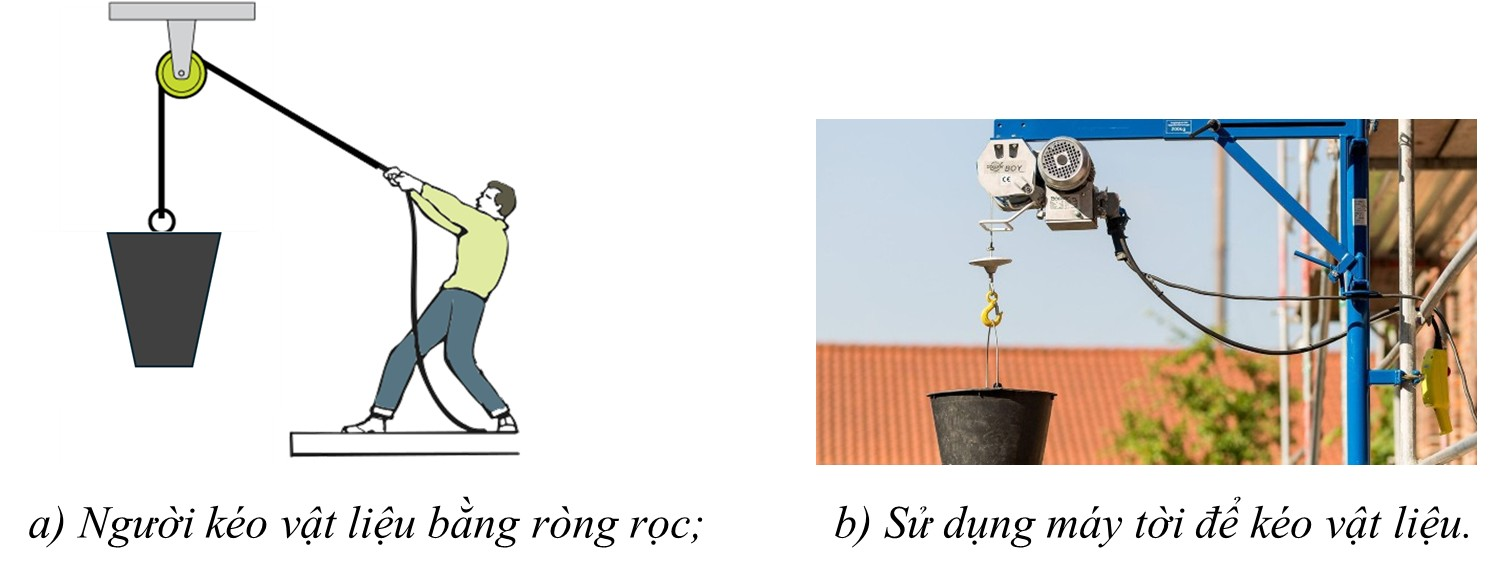
\includegraphics[scale=0.45]{../figs/D10-KTTX2-HK2-1}
	\end{center}
	\choiceTF
	{Khi đưa vật liệu lên cao bằng máy tời điện thì đã có sự chuyển hóa từ cơ năng sang điện năng}
	{\True Công tối thiểu cần thực hiện trong 2 trường hợp như nhau}
	{\True Khi kéo đều khối vật liệu thì công thực hiện của máy tời là \SI{5000}{\joule}}
	{\True Công suất kéo khối vật liệu của người và máy tời lần lượt là \SI{100}{\watt}, \SI{500}{\watt}}
	\loigiai{}
\end{ex}
% ===================================================================
\begin{ex}
	\immini{Một thang máy có khối lượng \SI{1.0E3}{\kilogram} có tải trọng tối đa \SI{8.0E2}{\kilogram}. Lực cản tác dụng lên thang máy không đổi và có độ lớn \SI{4.00E3}{\newton}. Thang máy đang chứa đầy tải trọng và đi lên đều với tốc độ \SI{3.0}{\meter/\second}.
	\choiceTF
	{Trong quá trình thang máy đi lên, trọng lực sinh công dương}
	{\True Độ lớn lực căng của dây cáp tác dụng lên thang máy là \SI{22}{\kilo\newton}}
	{\True Công suất trung bình của thang máy gần \SI{88.5}{HP}}
	{Motor thang máy hoạt động với công suất không đổi, nếu cần tăng độ lớn lực kéo của động cơ thì phải giảm tốc độ chuyển động của thang máy}
	}
	{\vspace{-0.65cm}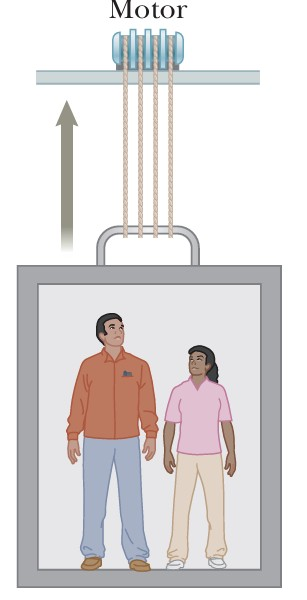
\includegraphics[scale=0.5]{../figs/D10-KTTX2-HK2-2}}
	
	\loigiai{}
\end{ex}
% ===================================================================
\begin{ex}
	\immini{Hình bên minh họa một vận động viên trượt tuyết đang tập luyện trên một con dốc có độ nghiêng $\theta=\SI{37}{\degree}$ và chân dốc được nối liền với đoạn đường nằm ngang một cách hoàn hảo (bỏ qua va chạm giữa giày trượt với đoạn nối chân dốc). Gió thổi từ đường hầm được sử dụng để giúp vận động viên điều chỉnh tư thế trong suốt quá trình trượt.}
	{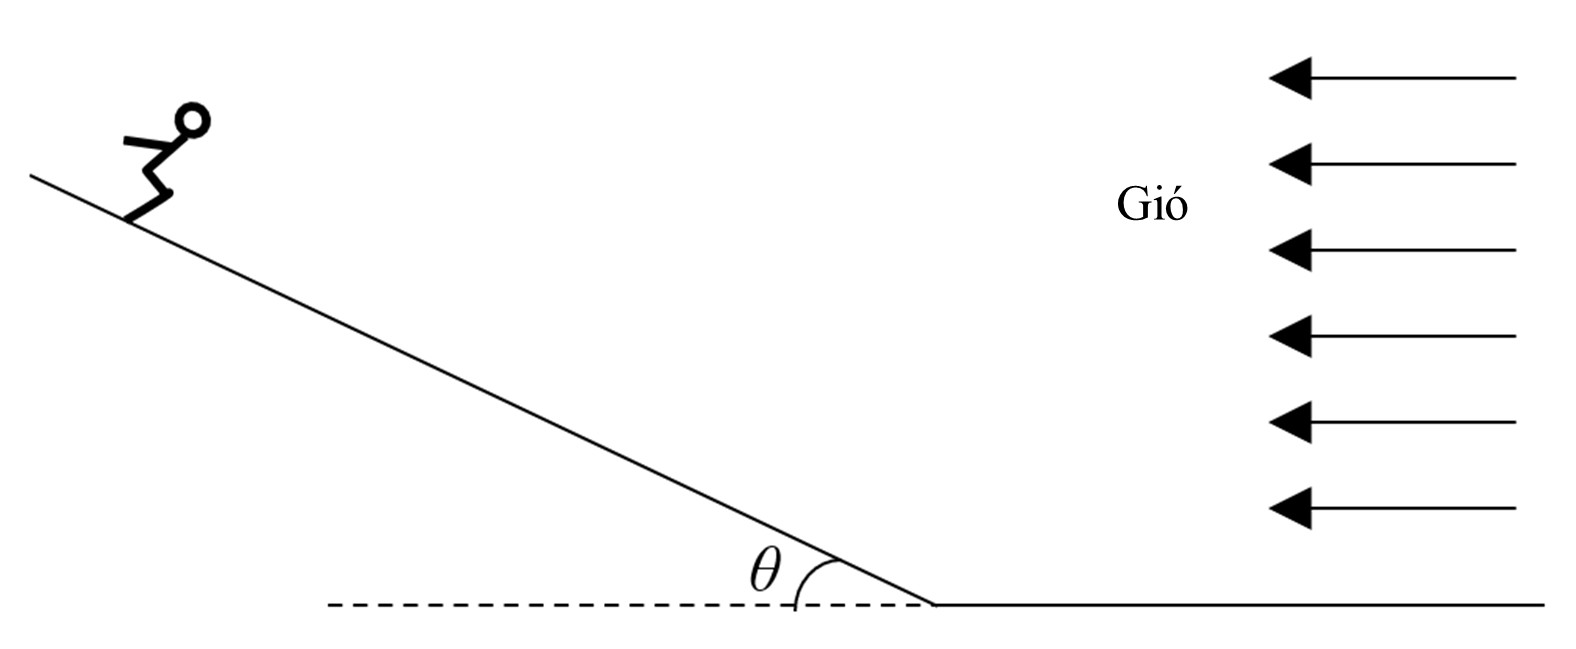
\includegraphics[scale=0.35]{../figs/D10-KTTX2-HK2-3}}
	Độ lớn lực cản do gió tạo ra tỉ lệ thuận với tốc độ tương đối của vận động viên với gió. Người này đi xuống dốc từ trạng thái nghỉ và đạt tốc độ không đổi \SI{25}{\meter/\second} khi anh ta xuống gần đến chân dốc. Sau khi đi đến mặt đường ngang, vận động viên tiếp tục trượt thêm \SI{50}{\meter} thì dừng lại. Biết rằng, vận động viên có khối lượng \SI{55}{\kilogram}, hệ số ma sát trượt giữa giày trượt với mặt dốc và mặt đường nằm ngang đều bằng \SI{0.3}{}.
	\choiceTF
	{Trong quá trình chuyển động trên mặt dốc, trọng lực tác dụng lên vận động viên không sinh công}
	{\True Trong quá trình chuyển động trên mặt dốc, lực do gió tác dụng lên người sinh công âm}
	{Khi người chuyển động với tốc độ không đổi trên dốc, độ lớn lực do gió tác dụng lên người là \SI{249.5}{\newton}}
	{\True Công của lực do gió tác dụng lên người trên đoạn đường nằm ngang là \SI{-8937.5}{\joule}}
	\loigiai{}
\end{ex}
\Closesolutionfile{ans}
\section{Tự luận}
\setcounter{ex}{0}
\Opensolutionfile{ans}[ans/D10-KTTX2-HK2-TL]
% ===============================================================
\begin{ex}
	Một gàu nước khối lượng \SI{10}{\kilogram} được kéo đều lên cao \SI{5}{\meter} trong khoảng thời gian \SI{1}{\minute} \SI{40}{\second}. Công suất trung bình của lực kéo bằng bao nhiêu watt $\left(\si{\watt}\right)$?
	\loigiai{
		\SI{5}{\watt}
	}
\end{ex}
% ===============================================================
\begin{ex}
	Một động cơ có công suất tiêu thụ điện bằng \SI{5}{\kilo\watt} kéo một vật có trọng lượng \SI{12}{\kilo\newton} lên cao \SI{30}{\meter} theo phương thẳng đứng trong thời gian \SI{90}{\second} với tốc độ không đổi. Hiệu suất của động cơ này bằng bao nhiêu \si{\percent}?
	\loigiai{
		\SI{80}{\percent}
	}
\end{ex}
% ===============================================================
\begin{ex}
	Một vật chuyển động đều trên mặt phẳng ngang trong một phút với tốc độ \SI{36}{\kilo\meter/\hour} dưới tác dụng của lực kéo \SI{20}{\newton} hợp với mặt phẳng ngang góc $\alpha=\SI{60}{\degree}$. Tính công và công suất của lực kéo trên.
	\loigiai{
		$A=\SI{6000}{\joule}$; $\calP=\SI{100}{\watt}$.
	}
\end{ex}
% ===============================================================
\begin{ex}
	Một vật có khối lượng $m=\SI{10}{\kilogram}$ trượt không vận tốc đầu từ đỉnh của một mặt phẳng nghiêng cao \SI{20}{\meter}. Khi tới chân dốc thì vật có tốc độ \SI{15}{\meter/\second}. Tính công của lực ma sát trong quá trình này theo đơn vị joule $\left(\si{\joule}\right)$.
	\loigiai{
		\SI{-875}{\joule}.
	}
\end{ex}
% ===============================================================
\begin{ex}
	Nhà máy thủy điện được xây dựng ở những nơi có thác nước cao để lợi dụng năng lượng nước chảy xuống. Tuabin nhà máy phát điện phát ra công suất \SI{25}{\mega\watt}. Biết mỗi phút nước chảy vào tuabin máy phát điện \SI{1800}{\meter^3} và hiệu suất của tuabin là \SI{80}{\percent}. Cho khối lượng riêng của nước là $\rho=\SI{1000}{\kilogram/\meter^3}$. Tính độ cao thác nước theo đơn vị mét $\left(\si{\meter}\right)$ và làm tròn kết quả đến chữ số hàng đơn vị.
	\loigiai{
		\SI{104}{\meter}.
	}
\end{ex}
% ===============================================================
\begin{ex}
	\immini{Một viên gạch có kích thước $a\times b\times c=6\times 10\times \SI{22}{\centi\meter^3}$ làm bằng vật liệu có khối lượng riêng \SI{2500}{\kilogram/\meter^3}. Hãy xác định công cần thiết để đưa viên gạch từ tư thế nằm ngang với diện tích đáy $b\times c$ sang tư thế thẳng đứng với diện tích đáy $a\times b$. Kết quả tính theo đơn vị joule $\left(\si{\joule}\right)$.}
	{\vspace{-0.5cm}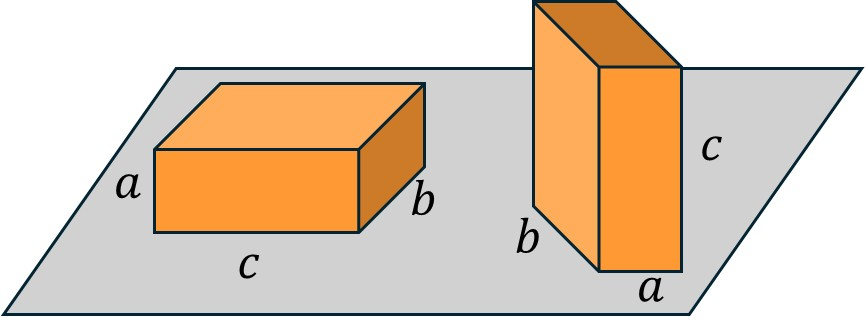
\includegraphics[scale=0.4]{../figs/D10-KTTX2-HK2-4}}
	\loigiai{
		\SI{2.64}{\joule}.
	}
\end{ex}
\Closesolutionfile{ans}
\begin{center}
	\textbf{--- HẾT ---}
\end{center}
\newpage
\begin{center}
	\textbf{\color{purple}QUÀ TẶNG KÈM \LARGE\smiley}
\end{center}
\setcounter{ex}{0}
\Opensolutionfile{ans}[ans/D10-KTTX2-HK2-BS]
% ===============================================================
\begin{ex}
	Một vật có khối lượng \SI{5}{\kilogram} được kéo đều trên quãng đường \SI{4}{\meter} với tốc độ không đổi lên phía trên đỉnh của một mặt phẳng nghiêng góc \SI{37}{\degree} so với mặt nằm ngang. Biết hệ số ma sát trượt là \SI{0.25}{}. Cho $\sin\SI{37}{\degree}=0,6$. Tính
	\begin{enumerate}[label=\alph*)]
		\item Công của trọng lực.
		\item Công của lực ma sát.
		\item Công của lực kéo.
	\end{enumerate}
	\loigiai{
		
	}
\end{ex}
% ===============================================================
\begin{ex}
	Một buồng thang máy có trọng lượng $P=\SI{2000}{\newton}$ và mang một vật có trọng lượng $Q=\SI{5000}{\newton}$. Thang máy đi lên đều trong 20 giây và lên cao được \SI{50}{\meter}.
	\begin{enumerate}[label=\alph*)]
		\item Tính công suất của động cơ thang máy.
		\item Nếu giữ nguyên công suất này và muốn lên cao được \SI{50}{\meter} trong thời gian \SI{10}{\second} thì trọng lượng tối đa của vật có thể bằng bao nhiêu?
	\end{enumerate}
	\loigiai{
		
	}
\end{ex}
% ===============================================================
\begin{ex}
	\immini{Đồ thị hình bên biểu diễn lực tác dụng của người công nhân thay đổi trong quá trình kéo bao tải trên mặt phẳng nghiêng và độ dịch chuyển trong ứng theo phương của lực. Tính công của người công nhân.}
	{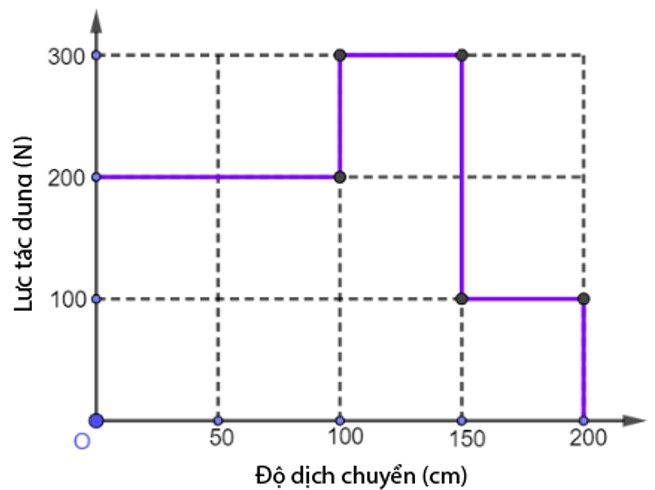
\includegraphics[scale=0.5]{../figs/D10-KTTX2-HK2-5}}
	\loigiai{
		
	}
\end{ex}
% ===============================================================
\begin{ex}
Một máy bơm nước có công suất \SI{1.5}{\kilo\watt}, hiệu suất \SI{70}{\percent}. Dùng máy này để bơm nước lên độ cao \SI{10}{\meter}, sau nửa giờ máy đã bơm lên bể một lượng nước bằng bao nhiêu $\si{\meter^3}$?
	\loigiai{
		
	}
\end{ex}
% ===============================================================
\begin{ex}
	Một người nặng \SI{60}{\kilogram} đi lên một cầu thang gồm $n$ bậc, mỗi bậc cao \SI{18}{\centi\meter}, dài \SI{24}{\centi\meter}. Coi lực mà người này tác dụng lên mỗi bậc thang là không đổi trong quá trình di chuyển. Công tối thiểu mà người ấy phải di thực hiện bằng $\SI{1.62}{\kilo\joule}$. Tìm số bậc thang $n$.
	\loigiai{
		
	}
\end{ex}
\Opensolutionfile{ans}